\documentclass[12pt]{article}
\usepackage{tikz}
\usetikzlibrary{bayesnet}
\usepackage{amsmath}
\begin{document}

\section*{Variational Inference Notes}

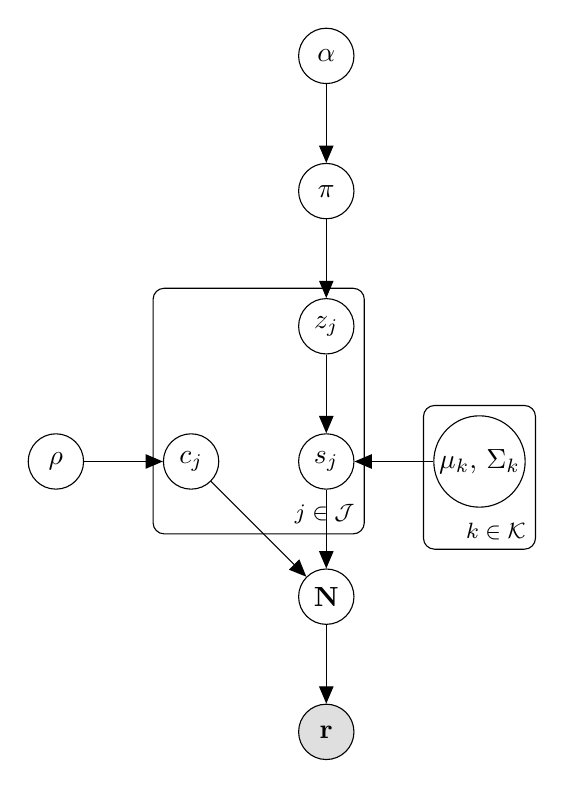
\begin{tikzpicture}

  % Define nodes
  \node[obs]                               (r) {$\mathbf{r}$};
  \node[latent, above=of r]        (N) {$\mathbf{N}$};
  \node[latent, above=of N] (s) {$s_j$};
  \node[latent, above=of s] (z) {$z_j$};
  \node[latent, above=of z] (pi) {$\pi$};
  \node[latent, above=of pi] (a) {$\alpha$};
  \node[latent, right=of s]  (th) {$\mu_k$, $\Sigma_k$};
  \node[latent, left=of s]  (c) {$c_j$};
  \node[latent, left=of c]  (rho) {$\rho$};
  % Connect the nodes
  \edge {c,s} {N};
  \edge {N} {r}; 
  \edge {rho} {c}; 
  \edge {pi} {z};
  \edge {a} {pi};
  \edge {z, th} {s}; 
  \plate {} {(c) (s) (z)} {$j \in \mathcal{J}$};
  \plate {} {(th)} {$k \in \mathcal{K}$};

\end{tikzpicture}
\\
$s_j|z_j \sim \mathcal{N}(\mu_{z_j}, \Lambda_{z_j})$\\
$N_{ij}|\{s_j\}  \sim \text{Poisson}(c_j f_i(s_j))$\\
$r_i|N_{ij} \sim \delta(r_i - \sum_j N_{ij})$\\
$\pi \sim \text{Dir} (\alpha)$\\
$c \sim \text{Dir} (\rho)$\\
\\
\begin{equation}
\begin{aligned}
\log Q(z) &= \langle \log P(z, s, c, \mu, \Lambda, N, r) \rangle_{Q(s)Q(N)Q(c)Q(\mu, \Sigma)}\\
&= \langle \log(\text{Mult}(z; \pi) \text{Dir}(\pi; \alpha) \prod_{j=1}^J \mathcal{N}(s_j; \mu_{z_j}, \Lambda_{z_j}) \text{Dir}(c, \rho)...\\
& \phantom{{}=1} \prod_{j=1}^J ((\delta(r_i - \sum_j N_{ij}) \text{Poisson}(c_j f_i(s_j)))...\\
& \phantom{{}=1} \prod_{k=1}^K \mathcal{N}(\mu_k; m_k, (\beta_0 \Lambda_k)) \mathcal{W}(\Lambda_k; \textbf{W}_0 ,\nu_0)) \rangle_{Q(s)Q(N)Q(c)Q(\mu, \Lambda)}\\
\log Q(z_j = k) &= \langle \log(\text{Mult}(z; \pi) \rangle_{Q(\pi)} + \langle \log (\prod_{j=1}^J \mathcal{N}(s_j; \mu_{z_j}, \Lambda_{z_j}) \rangle_{Q(s)Q(\mu, \Lambda)})\\
&= \frac{D}{2} \langle \log (|\Lambda_k|) \rangle_{Q(\Lambda)} - \frac{1}{2} \langle (s_j - \mu_k)^T \Lambda_k (s_k - \mu_k) \rangle_{Q(s)Q(\mu, \Lambda)} + \langle \log \pi_k \rangle_{Q(\pi)}\\
&= \frac{D}{2} (\sum_{d=1}^D \Psi (\frac{\nu_k^* + 1 - d}{2}) + \log (|\textbf{W}_k^*|))\\
& \phantom{{}=1} - \frac{1}{2} (D \beta_k^{*^{-1}} + \nu_k^* ((\mu_k^* - m_j^*)^T \textbf{W}_k^* (\mu_k^* - m_j^*)) + \text{Tr}(\textbf{W}_k^* \Lambda_j^{*^{-1}}))\\
& \phantom{{}=1} + \Psi(\alpha_k) - \Psi(\sum_{k=1}^K \alpha_k)\\
q_{jk}^* &= \frac{Q(z_j = k)}{\sum_{k=1}^K Q(z_j = k)}
\end{aligned}
\end{equation}
\\
\begin{equation}
\begin{aligned}
\log Q(c) &= \langle \sum_j (\rho_j - 1) \log c_j \rangle + \sum_{ij} \langle N_{ij} \log c_j \rangle \\
&= \sum_j [\log c_j][\rho_j - 1 + \sum_i \langle N_{ij} \rangle]\\
Q(c) &\sim \text{Dir}(\rho_j - 1 + \sum_i \langle N_{ij} \rangle) = \text{Dir}(\gamma_j^*)\\
\gamma_j^* &= \rho_j - 1 + \sum_i r_i p^*_{ij}\\
\langle \log c_j \rangle &= \Psi(\rho_j - 1 + \sum_i r_i p^*_{ij}) - \Psi(\sum_j (\rho_j - 1 + \sum_i r_i p^*_{ij}))
\end{aligned}
\end{equation}
\\
\begin{equation}
\begin{aligned}
\log Q(s_j) &= \langle \log \mathcal{N}(\mu_{z_j}, \Lambda_{z_j}) \rangle_{Q(z)Q(\mu, \Lambda)} + \sum_{i=1}^I \langle N_{ij} \log f_i(s_j) \rangle_{Q(N)}\\
&= - \frac{1}{2} (\langle (s_j - \mu_j)^T \Lambda_{z_j}^{-1} (s_j - \mu_j) \rangle_{Q(z)Q(\mu, \Lambda)} + \sum_{i=1}^I \langle N_{ij} \rangle_{Q(N)} \log f_i(s_j))\\
&= - \frac{1}{2} (\sum_{k=1}^K q_{jk}^* \nu^*_k (s_j - \mu_k)^T \mathbf{W}^*_k (s_j - \mu_k) - \frac{1}{2} \sum_{i=1}^I 2 \frac{||s_j - s_i^{\text{pref}}||^2}{2 \sigma^2})\\
Q(s_j) &\sim \mathcal{N} (m^*_j, \Lambda^*_j)\\
\Lambda^*_j &= \sum_{l=1}^{K+I} \Lambda_l\\
m^*_j &= \Lambda^*_j \sum_{l=1}^{K+I} (\Lambda_l m_l)\\
m_l &\in \{m_k\}_{k=1}^K, \{s_i^{\text{pref}}\}_{i=1}^I\\
\Lambda_l &\in \{ q_{kj}^* \nu^*_k \mathbf{W}^*_k \}_{k=1}^K, \{\frac{2 r_i p_{ij}}{2 \sigma^2}I\}_{i=1}^I\\
\langle \log f_i(s_j) \rangle_{Q(s_j)} &= \frac{- \langle ||s_j - s_i^{\text{pref}}||^2 \rangle_{Q(s_j)}}{2 \sigma^2}\\
&=  \frac{-||s_i^{\text{pref}} - m_j^*||^2 + \text{Tr}(\Lambda_j^{*^{-1}})}{2 \sigma^2}
\end{aligned}
\end{equation}
\\
\begin{equation}
\begin{aligned}
\log Q(N_i) &= \log(\delta(\sum_{j=1}^J N_{ij} -r_i)) + \sum_{j=1}^J N_{ij}[\langle \log c_j \rangle + \langle \log f_i(s_j) \rangle] - \sum_{j=1}^J \log N_{ij}!\\
Q(N_{ij}) &\sim \text{Mult}(r_i, p^*_{ij})\\
p^*_{ij} &= \frac{e^{\langle \log c_j \rangle + \langle \log f_i(s_j) \rangle}}{\sum_{j=1}^J e^{\langle \log c_j \rangle + \langle \log f_i(s_j) \rangle}}\\
&= \frac{e^{\Psi(\gamma_j^*) - \Psi(\sum_{j=1}^J \gamma_j^*) - \frac{||s_i^{\text{pref}} - m_j^*||^2 + \text{Tr}(\Lambda_j^{*^{-1}})}{2 \sigma^2}}}{\sum_{j=1}^J e^{\Psi(\gamma_j^*) - \Psi(\sum_{j=1}^J \gamma_j^*)  - \frac{||s_i^{\text{pref}} - m_j^*||^2 + \text{Tr}(\Lambda_j^{*^{-1}})}{2 \sigma^2}}}
\end{aligned}
\end{equation}
\\
\begin{equation}
\begin{aligned}
\log Q(\mu_k, \Lambda_k) &= \langle \log (\prod_{j=1}^J \mathcal{N}(s_j; \mu_{z_j}, \Lambda_{z_j}) \rangle_{Q(s)Q(z)})\\
&= \langle \sum_{j=1}^J [\frac{D}{2} \log |\Lambda_{z_j}| - \frac{1}{2}[(s_j - \mu_{z_j})^T \Lambda_{z_j} (s_j - \mu_{z_j}) \rangle_{Q(s)Q(z)}\\
&= \langle \sum_{j=1}^J [\frac{D}{2} \log |\Lambda_{z_j}| - \frac{1}{2}[(m^*_j - m_{z_j})^T \Lambda_{z_j} (m^*_j - m_{z_j}) + \text{Tr}(\Lambda_{z_j} \Lambda_j^{*^{-1}})] \rangle_{Q(z)}\\
&= \sum_{j=1}^J q_{jk}^* [\frac{D}{2} \log |\Lambda_{z_j}| - \frac{1}{2}[(m^*_j - m_{z_j})^T \Lambda_{z_j} (m^*_j - m_{z_j}) + \text{Tr}(\Lambda_{z_j} \Lambda_j^{*^{-1}})]\\
Q(\mu_k, \Lambda_k) &\sim \mathcal{N} (\mu_k; \mu^*_k, (\beta^*_k \Lambda_k)) \mathcal{W} (\Lambda_k; \mathbf{W}^*_k, \nu^*_k)\\
\sum_{j=1}^J q_{jk}^* \text{Tr} (\Lambda_k \Lambda_j^{*^{-1}}) &= \text{Tr} (\Lambda_k \sum_{j=1}^J q_{jk}^* \Lambda_j^{*^{-1}})\\
\mathbf{W}^*_k &= (\sum_{j=1}^J (q_{jk}^* \Lambda_j^{*^{-1}}))^{-1}\\
|\Lambda_{z_j}|^{\frac{\nu_k^* - 1}{2}} &= |\Lambda_{z_j}|^{\frac{D}{2} + \sum_{j=1}^J q_{jk}^*}\\
\nu_k^* &= D + 2 \sum_{j=1}^J q_{jk}^* + 1\\
C &= \Lambda_k \sum_{j=1}^J q_{jk}^*\\
X &= \Lambda_k \sum_{j=1}^J q_{jk}^* m_j^*\\
\mu^*_k &= \frac{X}{C} = \frac{\sum_{j=1}^J q_{jk}^*m_j^*}{\sum_{j=1}^J q_{jk}^*}\\
(\beta_k^* \Lambda_k)^{-1} &= C\\
\beta_k^* &= \frac{1}{\sum_{j=1}^J q_{jk}^*}\\
\end{aligned}
\end{equation}
\\
\begin{equation}
\begin{aligned}
\frac{d q_{jk}^*}{dt} &= - q_{jk}^* + \frac{Q(z_j = k)}{\sum_{k=1}^K Q(z_j = k)}\\
\frac{d m_j^*}{dt} &= - m_j^* + \Lambda^*_j (\sum_{k=1}^K (q_{kj}^* \nu^*_k \mathbf{W}^*_k \mu^*_k) + \sum_{i=1}^I (\frac{2 r_i p_{ij}}{2 \sigma^2} I s_i^{\text{pref}}))\\
\frac{d \Lambda^*_j}{dt} &= - \Lambda^*_j + \sum_{k=1}^K (q_{kj}^* \nu^*_k \mathbf{W}^*_k) + \sum_{i=1}^I (\frac{2 r_i p_{ij}}{2 \sigma^2}I)\\
\frac{d p_{ij}^*}{dt} &= - p_{ij}^* + \frac{e^{\Psi(\gamma_j^*) - \Psi(\sum_{j=1}^J \gamma_j^*) - \frac{||s_i^{\text{pref}} - m_j^*||^2 + \text{Tr}(\Lambda_j^{*^{-1}})}{2 \sigma^2}}}{\sum_{j=1}^J e^{\Psi(\gamma_j^*) - \Psi(\sum_{j=1}^J \gamma_j^*) - \frac{||s_i^{\text{pref}} - m_j^*||^2 + \text{Tr}(\Lambda_j^{*^{-1}})}{2 \sigma^2}}}\\
\frac{d \gamma_j^*}{dt} &= - \gamma_j^* + \rho_j - 1 + \sum_i r_i p^*_{ij}\\
\frac{d \mu_k^*}{dt} &= - \mu_k^* + \frac{\sum_{j=1}^J q_{jk}^*m_j^*}{\sum_{j=1}^J q_{jk}^*}\\
\frac{d \beta_k^*}{dt} &= - \beta_k^* + \frac{1}{\sum_{j=1}^J q_{jk}^*}\\
\frac{d \mathbf{W}^*_k}{dt} &= - \mathbf{W}^*_k + (\sum_{j=1}^J (q_{jk}^* \Lambda_j^{*^{-1}}))^{-1}\\
\frac{d \nu^*_k}{dt} &= - \nu^*_k + D + 2 \sum_{j=1}^J q_{jk}^* + 1
\end{aligned}
\end{equation}
\end{document}